\section{Context as a Derivative}

\begin{frame}[fragile]
\frametitle{Context Examples Recap}

\begin{itemize}[<+->]
\item
\begin{lstlisting}
'a list = unit + 'a * 'a list
'a list_context = 'a list * 'a list
\end{lstlisting}

\item
\begin{lstlisting}
'a btree = unit + 'a * 'a btree * 'a btree
'a btree_context = 'a btree * 'a btree
           * (bool * 'a * 'a btree) list
\end{lstlisting}

\item 
\begin{lstlisting}
'a tree = unit + 'a * a tree list
'a tree_context = 'a tree list
           * ('a tree list * 'a * 'a tree list) list
\end{lstlisting}

\item Math-ly notation, e.g. $\Flist (a) = 1 + a \times \Flist (a)$

\item Context for an arbitrary algebraic data type?
\end{itemize}
\end{frame}

\begin{frame}[fragile]
\frametitle{Context of Basic Types}

\begin{itemize}[<+->]
\item Note the context of type $a$ inside type $T$ by $C[a](T)$
\begin{itemize}
\item e.g. $C[a](\Flist(a)) = \Fdlist(a) = \Flist(a) \times \Flist(a)$
\end{itemize}

\item Context of type $a$ inside type $1$ (i.e. \lstinline|unit|): impossible!
\begin{itemize}
\item $C[a](1) = 0$
\end{itemize}

\item Context of type $a$ inside type $a$: dummy unit
\begin{itemize}
\item $C[a](a) = 1$
\end{itemize}
\end{itemize}
\end{frame}

\begin{frame}
\frametitle{Context of Sum Type}
\begin{itemize}
\item Inside $T_1 + T_2$, type $a$ occurs in either of them
\begin{itemize}
\item $C[a](T_1+T_2) = C[a](T_1) + C[a](T_2)$
\end{itemize}
\end{itemize}

\begin{figure}
\centering

\includegraphics[width=\textwidth]{figure/sum}
\end{figure}
\end{frame}

\begin{frame}
\frametitle{Context of Product Type}
\begin{itemize}
\item Inside $T_1 \times T_2$, type $a$ occurs in one of them,
while the other must be carried in the context
\begin{itemize}
\item $C[a](T_1\times T_2) = C[a](T_1)\times T_2 + T_1\times C[a](T_2)$
content
\end{itemize}
\end{itemize}

\begin{figure}
\centering
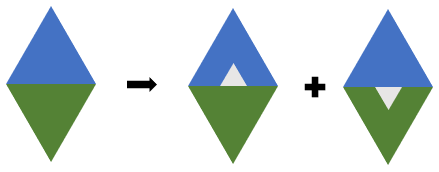
\includegraphics[width=\textwidth]{figure/prod}
\end{figure}
\end{frame}

\begin{frame}
\frametitle{Context of Composed Type}

\begin{itemize}
\item Inside composed type $T(U(a))$, type $a$ occurs in one of $U$,
which resides somewhere in $T$
\begin{itemize}
\item $C[a](T(U(a))) = C[b](T(b))|_{b=U(a)} \times  C[a](U(a))$
\end{itemize}
\end{itemize}

\begin{figure}
\centering
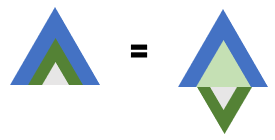
\includegraphics[width=0.7\textwidth]{figure/comp}
\end{figure}
\end{frame}

\begin{frame}
\frametitle{Context as Derivative}
\begin{itemize}
\item Rules for context:
\begin{itemize}
\item $C[a](1) = 0$
\item $C[a](a) = 1$
\item $C[a](T_1 + T_2) = C[a](T_1) + C[a](T_2)$
\item $C[a](T_1 \times  T_2) = C[a](T_1)\times T_2 + T_1\times C[a](T_2)$
\item $C[a](T(U(a))) = C[b](T(b))|_{b=U(a)} \times  C[a](U(a))$
\end{itemize}

\item Rules for derivative:
\begin{itemize}
\item $\frac{\partial}{\partial x}c = 0$
\item $\frac{\partial}{\partial x}x = 1$
\item $\frac{\partial}{\partial x}(f+g) = \frac{\partial}{\partial x}f + \frac{\partial}{\partial x}g$
\item $\frac{\partial}{\partial x}(f\cdot g) = \frac{\partial}{\partial x}f \cdot g
+ f \cdot \frac{\partial}{\partial x}g$
\item $\frac{\partial}{\partial x}(f\circ g)|_{x_0} =
\frac{\partial}{\partial u}f|_{u=g(x_0)}
\cdot \frac{\partial}{\partial x}g|_{x=x_0}$
\end{itemize}

\item $\Pa (T) \triangleq C[a](T)$
\end{itemize}
\end{frame}

%%%% begin [deriv list] %%%%
\begin{frame}
\frametitle{Context of List, Revisit}

\begin{align*}
\onslide<+->{\Pa \Flist(a)
&=\Pa (1+a \times \Flist(a))\\}
\onslide<+->{&=0 + \Pa (a \times \Flist(a))\\}
\onslide<+->{&=\Flist(a) + a \times \Pa \Flist(a)\\}
\onslide<+->{\Pa \Flist(a) &= \Flist(a) \times \Flist(a)\\}
\onslide<+->{&= \Fdlist(a)}
\end{align*}
\end{frame}
%%%% end [deriv list] %%%%

%%%% begin [deriv btree] %%%%
\begin{frame}
\frametitle{Binary Tree Context Revisit}

\begin{align*}
\onslide<+->{\Pa \Fbtree(a)
&= \Pa (1 + a \times \Fbtree^2(a)) \\}
\onslide<+->{
&=0
+ \Pa (a \times \Fbtree^2(a)) \\}
\onslide<+->{
&=\Fbtree^2(a)
+ a \times \Pa \Fbtree^2(a) \\}
\onslide<+->{
&=\Fbtree^2(a)
+ a \times 2 \times \Fbtree(a) \times \Pa \Fbtree(a) \\}
\onslide<+->{\Pa \Fbtree(a)
&= \Fbtree^2(a) \times \Flist (2 \times a \times \Fbtree(a)) \\}
\onslide<+->{
&= \Fdbtree(a)}
\end{align*}
\end{frame}
%%%% end [deriv btree] %%%%

%%%% begin [deriv tree] %%%%
\begin{frame}
\frametitle{Context of Tree, Revisit}
\begin{align*}
\onslide<+->{\Pa\Ftree(a)
&= \Pa(1 + a \times \Flist(\Ftree(a)))
\\}
\onslide<+->{
&= 0 + \Pa(a \times \Flist(\Ftree(a)))
\\}
\onslide<+->{
&=  \Flist(\Ftree(a)) + a \times \Pa(\Flist(\Ftree(a)))
\\}
\onslide<+->{
&= \Flist(\Ftree(a)) + a \times \Flist^2(\Ftree(a)) \times \Pa(\Ftree(a))
\\}
\onslide<+->{\Pa \Ftree(a)
&= \Flist(\Ftree(a)) \times \Flist(a \times \Flist^2(\Ftree(a)))
\\}
\onslide<+->{
&= \Fdtree(a)
\\}
\end{align*}
\end{frame}
%%%% end [deriv tree] %%%%

%%%% begin [deriv ltree] %%%%
\begin{frame}
\frametitle{Huet's Zipper, Revisit}

\begin{itemize}
\item $\Fltree(a) = a + \Flist(\Fltree(a))$
\item Differentiating against non-basic type is a bit tricky
\item $\frac{\partial}{\partial \Fltree}(\Fltree) = 1$?
\item $\frac{\partial}{\partial \Fltree}(\Fltree) = \frac{\partial}{\partial \Fltree}(a + \Flist(\Fltree))$?
\item A hack:
$\begin{aligned}[t]
\frac{\partial}{\partial \Fltree}
&= \mathbf{((1))} + \frac{\partial}{\partial \Fltree}(
a + \Flist(\Fltree))\\
&= \mathbf{1} + \frac{\partial}{\partial \Fltree}(\Flist(\Fltree))\\
&= \mathbf{1} + \Flist^2(\Fltree) \times \frac{\partial}{\partial \Fltree}(\Fltree) \\
&= \Fdltree
\end{aligned}$
\end{itemize}
\end{frame}
%%%% end [deriv ltree] %%%%

%%%% begin [rev] %%%%
\begin{frame}
\begin{itemize}
\item $\Pa \Ftree(a) = \Flist(\Ftree(a)) \times \Flist(a \times \Flist^2(\Ftree(a)))$
\item Reversed interpretation of the recursion path:
\end{itemize}

\bigskip

\begin{columns}
\begin{column}{0.4\textwidth}
\centering
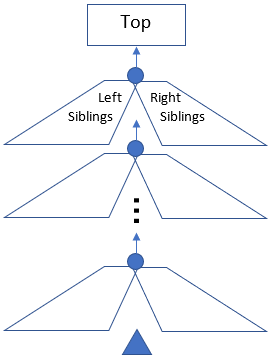
\includegraphics[width=\textwidth]{figure/zipper}
\end{column}

\begin{column}{0.4\textwidth}
\centering
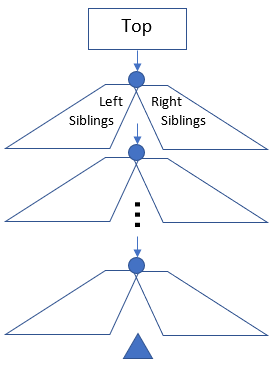
\includegraphics[width=\textwidth]{figure/zipper_rev}
\end{column}
\end{columns}
\end{frame}
%%%% end [rev] %%%%

%%%% begin [listexp] %%%%
\begin{frame}
\frametitle{Subtraction and Division?}

\begin{itemize}[<+->]
\item $\Flist(a) = 1 + a \times \Flist(a)$
\item $\Flist(a) \leftrightarrow \frac{1}{1-a}$?
\item $\Pa\Flist(a) \leftrightarrow \Pa(\frac{1}{1-a})
= \frac{1}{(1-a)^2} \leftrightarrow \Flist^2(a)$ ?!
\end{itemize}
\end{frame}
%%%% end [listexp] %%%%